%File: formatting-instruction.tex
\documentclass[letterpaper]{article}
\usepackage{aaai}
\usepackage{times}
\usepackage{helvet}
\usepackage{courier}
\usepackage{amsmath}
\usepackage{graphicx}
\usepackage{subfig}
\frenchspacing
\setlength{\pdfpagewidth}{8.5in}
\setlength{\pdfpageheight}{11in}
% \pdfinfo{
% /Title (Comparison of Spatial Relations Based Object Classification and Scene Understanding Techniques Using a Large Annotated 3D Scene-Object Dataset)
% /Author (Akshaya, Chris, Lars, Marina, Rares, John, Patric, Nick)}
% UNCOMMMENT:
%\setcounter{secnumdepth}{0}
%\usepackage{color}

% Self Included Packages:
% -----------------------
\setcounter{secnumdepth}{2}

% Set to \draftfalse if you want to remove points and ideas 
\newif\ifdraft
% \drafttrue
\draftfalse



\ifdraft
\newcommand{\lars}[1]{\textcolor{blue}{Lars:\ #1}}
\newcommand{\akshaya}[1]{\textcolor{Green}{Aks:\ #1}}
\newcommand{\chris}[1]{\textcolor{RedOrange}{Chr:\ #1}}
\newcommand{\marina}[1]{\textcolor{Purple}{Mar:\ #1}}
\newcommand{\rares}[1]{\textcolor{Aquamarine}{Rar:\ #1}}
\newcommand{\john}[1]{\textcolor{RubineRed}{Jon:\ #1}}
\newcommand{\patric}[1]{\textcolor{Red}{Pat:\ #1}}
\newcommand{\nick}[1]{\textcolor{Aquamarine}{Nick:\ #1}}
\newcommand{\points}[1]{\textcolor{Gray}{points-to-remember:\ #1}}
\else
\newcommand{\lars}[1]{}
\newcommand{\akshaya}[1]{}
\newcommand{\chris}[1]{}
\newcommand{\marina}[1]{}
\newcommand{\rares}[1]{}
\newcommand{\john}[1]{}
\newcommand{\patric}[1]{}
\newcommand{\nick}[1]{}
\newcommand{\points}[1]{}
\fi

\usepackage[usenames,dvipsnames]{color}
% ----------------------
 \begin{document}
% The file aaai.sty is the style file for AAAI Press 
% proceedings, working notes, and technical reports.
%
\title{A Comparison of Spatial Relation Models for Scene Understanding}
% \author{Akshaya, Chris, Lars, Marina, Rares, John, Patric, Nick\\
% KTH Royal Institute of Technology\\
% University of Birmingham
% }
\maketitle
\begin{abstract}
\begin{quote}

Object recognition approaches can be unreliable when run in isolation, but their performance can be improved when taking \emph{scene context} into account. In this paper, we present techniques to model and infer object labels in real scenes based on a variety of \emph{spatial relations} -- geometric features which capture \textit{how} objects co-occur -- and compare their efficacy in the context of augmenting perception based object classification in real-world table-top scenes. We also contribute a novel, large, periodic, long-term dataset of 20 3D table-top scenes, collected over 19 days, three times a day and manually annotated with 18 object classes. On this dataset, we show that more intricate techniques, have a superior performance but do not generalise well on small training data. We also show that techniques using coarser information perform crudely but sufficiently well in standalone scenarios and generalise well on small training data.
\end{quote}
\end{abstract}

\section{Introduction}
\label{sec:Introduction}

Objects pervade human environments. If robots are to perform useful service tasks for humans it is crucial that they are able to locate and identify a wide variety of objects in everyday environments. State-of-the-art object recognition/classification typically relies on the extraction features to be matched against models built through machine learning techniques. As - the number of objects a given system is trained to recognise - increases, the uncertainty of individual recognition results tends to increase as greater number of objects increases the chance of overlapping features existence. The reliability of such recognisers is also affected when used on real robots in everyday environments, as objects may be partially occluded by scene clutter or only visible from certain angles, both potentially reducing the visibility of features for their trained models. In this paper we argue that the performance of a robot on an object recognition task can be increased by the addition of \emph{contextual knowledge} about the scene the objects are found in. In particular we demonstrate how models of the \emph{spatial configuration} of objects, learnt over prior observations of real scenes, can allow a robot to recognise the objects in unseen scenes more reliably. 

Our work is performed in the context of developing a mobile service robot for long-term autonomy in indoor human environments, from offices to hospitals. The ability for a robot to run for weeks or months in its task environment opens up a new range of possibilities in terms of capabilities. In particular, any task the robot performs will be done in an environment it may have visited many times before, and we wish to find ways to capture the contextual knowledge gained from previous visits in a way that enables subsequent behaviour to be improved. The use of context to improve object recognition is just one example of this new robotics paradigm. In this paper we focus on the task of \emph{table-top scene understanding}, and more specifically what objects are present on a table-top. Whilst the objects present on a single table may change in position, their overall arrangement has some regularity over time as influenced by the use to which the table is put. For example, if this table is used for computing, then a (relatively static) monitor will be present, with a keyboard in front of it and mouse to one side. A drink, or paper and a pen, may be within an arms length of the keyboard, as may headphones or a cellphone. This arrangement may vary across different tables in the same building, but the overall pattern of arrangements will contain some structure. It is this structure we aim to exploit in order to improve the recognition of table-top objects, e.g. knowing that the object to the right of a keyboard is more likely to be a mouse than a cellphone. 

As the absolute positions of objects on a table (or their relative positions with respect to some fixed part of the table) is unlikely to generalise across a range of different tables, we are investigating \emph{relational} models of space, i.e. ways of encoding the position of a target object relative to the position of one or more landmark objects. Using a novel data set of table-top scenes (described in Section~\ref{sec:Dataset}), in this paper we explore the performance of a variety of representations for relative object position, plus inference techniquess for operating on them, on the task of table-top scene understanding (Section \ref{sec:Techniques}). In particular we investigate representations that use varying forms of spatial relations, from geometric ones such as distances and angles to more qualitative spatial relations such as \textit{Left} and \textit{Behind} as a means for capturing observations of object configurations over time. The contributions this paper makes are: (1) A novel comparison between mechanisms for representing, learning and inference on object spatial configurations using spatial relations. (2) An evaluation of the use of these mechanisms for augmenting a robot's vision based \textit{perceptual system} (PS). (3) A new large 3D annotated table-top benchmark dataset.

\ifdraft
\points{
\subsubsection*{Points discussed}
\begin{enumerate}
	\item Overview of the problem - why?
	\begin{enumerate}
		\item Not only table-tops
		\item How do we treat object classification
	\end{enumerate}
	\item Generalize and Transfer Knowledge
	\item How are objects correlated, search becomes easier
	\item Understanding a model for inter object influence for inference
	\item No benchmarks yet or datasets having 3D spatial information
	\begin{itemize}
		\item time
		\item complete scenes
		\item different people
		\item different types of people
	\end{itemize}
	\item need to structure data -- metric is tedious, because of large amounts of data
	\item Contributions:
	\begin{itemize}
		\item A big 3D data set, annotated -- benchmark for results, folding data, classification.
		\item suggest SM and QSR
		\item something that could augment perception systems
	\end{itemize}
\end{enumerate}
}
\fi

\section{Related Work}
\label{sec:Related Work}
\subsection{Spatial Relations Based Techniques}

Spatial relations have been used previously to provide contextual information to vision-related work. \citeauthor{MyungJin:CVPR2010}~\shortcite{MyungJin:CVPR2010} used a hierarchy of spatial relations alongside descriptive features to support multiple object detections in a single image. Spatial relations and contextual information are commonly used in activity recognition from video streams. For example, \citeauthor{Krishna:ECAI2010}~\shortcite{Krishna:ECAI2010} demonstrate the learning of activity phases in airport videos using spatial relations between tracked objects, and \citeauthor{Behera2012}~\shortcite{Behera2012} use spatial relations to monitor objects and activities in videos of a constrained workflow environment. Recent work has used object co-occurrence to provide context in visual  tasks. Examples in 2D include object co-occurrence statistics in class-based image segmentation~\cite{Ladicky:IJCV2013}; and the use of object presence to provide context in activity recognition~\cite{Li:2012}. However, all this previous work is restricted to 2D images, whereas our approaches work with spatial context in 3D (RGB-D) data. Authors have also worked with spatial context in 3D, including parsing a 2D image of a 3D scene into a simulated 3D field before extracting geometric and contextual features between the objects \cite{Xiao:SIGGRAPH2012}. Our approaches to encoding 3D spatial context could be applied in these cases, and we use richer, structured models of object relations.

Apart from using the statistics of co-occurrence, a lot of information can be exploited from \textit{how} the objects co-occur in the scene, i.e. the extrinsic, geometric spatial relations between the objects. Recent work in 3D semantic labelling has used such geometric information along with descriptive intrinsic appearance features~\cite{Koppula:NIPS2011}. They achieve a high classification accuracy for a large set of object-classes belonging to home and office environments. Scene similarity measurement and classification based on contextual information is conducted by \cite{Fisher:ACMT2011}. They also use spatial information for context-based object search using Graph Kernel Methods. The method is further developed to provide synthetic scene examples using spatial relations \cite{Fisher:ACMT2012}. In~\cite{Aydemir:ICRA2011} spatial relations between smaller objects, furniture and locations is used for pruning in object search problems in human environments. In \cite{Lin:ICCV2013} a technique is developed for automatic annotation of 3D objects. It uses intrinsic appearance features and geometric features and is employed to build an object and scene classifier using conditional random fields. In \cite{kasper:2011} the authors utilise both geometric single object features and pair-wise spatial relations between objects to develop an empirical base for scene understanding. Recent studies \cite{Southey:2007,kasper:2011} compute statistics of spatial relations of objects and use it for conditional object recognition for service robotics. Whilst our techniques are comparable to those in the literature, our contribution comes from the explicit comparison of different representations of spatial context (metric vs qualitative) on a novel, long-term learning task. Additionally our qualitative approach relies on relationships which could be provided through other mechanisms than unsupervised machine learning (e.g. through a human tutor describing a spatial scene), and in this way bootstrap the system using expert knowledge.

Our work is evaluated on a new 3D long-term dataset. Other datasets exist: The \textit{B3DO dataset} \cite{Janoch:ICCV2011} which contains many single-snapshot instances of indoor human environments having a variety in viewpoints, object-classes, scene-classes and instances. This dataset is in the form of RGB and depth image pairs with manual 2D annotations of object classes, capturing many unique scenes with the sole aim of finding more realistic scenes which are difficult for PSs to perform scene classification. \textit{NYU Depth V1-2} \cite{Silberman:ECCV2012} datasets contain different instance examples of object-classes and scene-classes. Each image instance is a combo of synchronous RGB and D images of a different scene-class with semantic annotation provided to every pixel. This dataset is aimed at helping PSs with automatic semantic segmentation and scene classification. The \textit{3D IKEA database} \cite{Swadzba:RAS2012} has been collected using robotic maneuvering in different scene-class instances. The aim is to test scene-classification algorithms based on large furniture level objects. The \textit{WRGBD dataset} \cite{Lai:ICRA2011} is aimed to support object classification methods and contains many instances of isolated objects in .pcd format. Annotation is done by assigning every pixel a correct semantic label.None of these datasets contain periodically collected data or easily usable spatial annotations of objects which are key for long-term autonomous scene-learning, based on spatial relations.


\ifdraft
\points{
\begin{enumerate}
	\item QSR - LEEDS activity recognition
	\item Datasets out there and why we cannot use them
	\item State of art object classification / single object classification
	\item Constellations or group estimation
	\item Object search from CAS
\end{enumerate}
}
\fi
\section{Dataset}
\label{sec:Dataset}
\begin{figure}[t]
%\captionsetup[subfigure]{labelformat=empty}
\begin{center}
\subfloat[][]{\label{fig:HistOfObjects}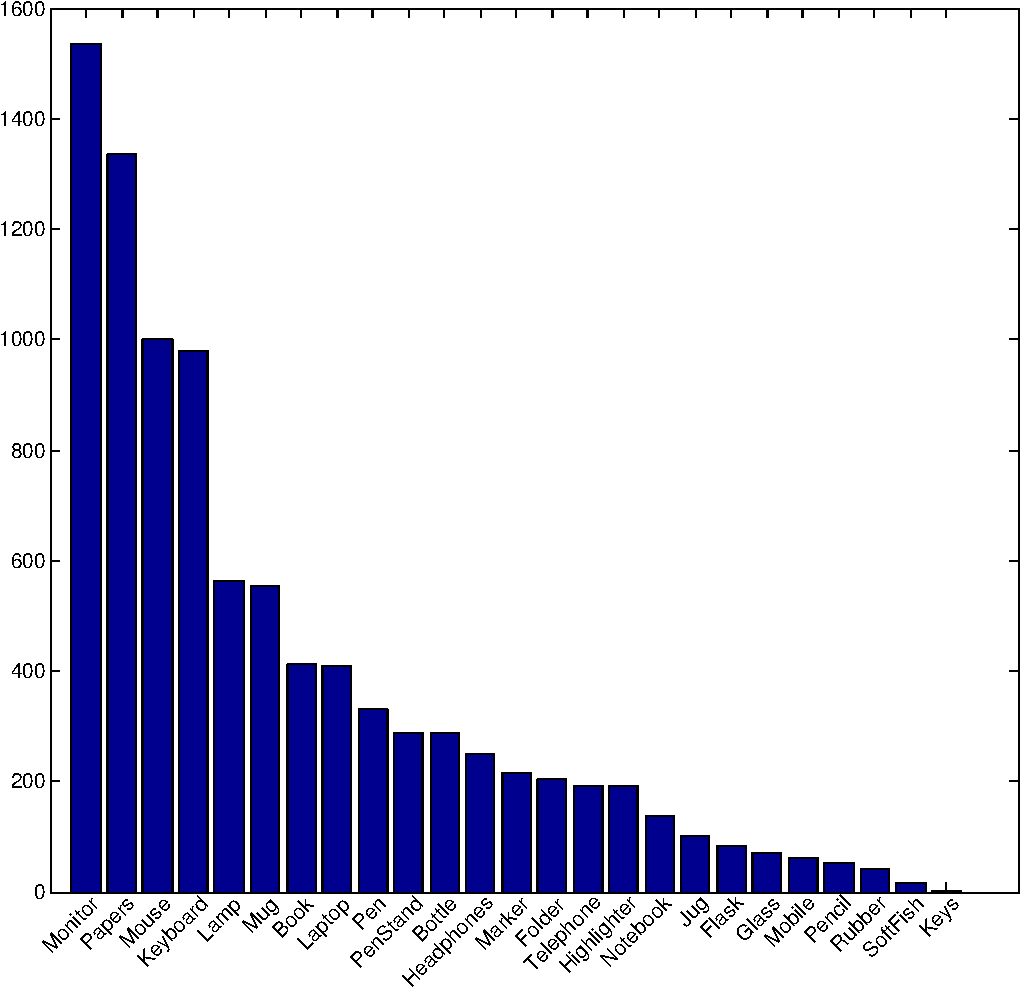
\includegraphics[scale=0.25]{HistOfObjects_crp.pdf}}\quad
\subfloat[][]{\label{fig:RawPCD}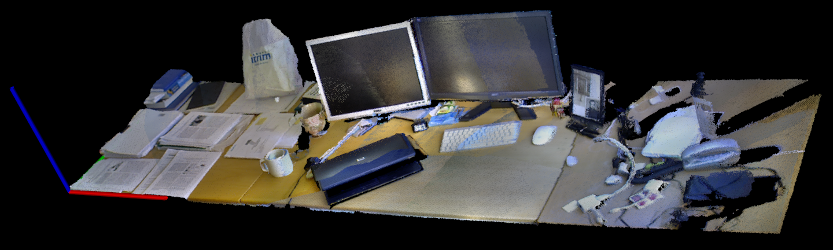
\includegraphics[scale=0.1]{pcd.png}}\\
\subfloat[][]{\label{fig:RawPCDAnnotated}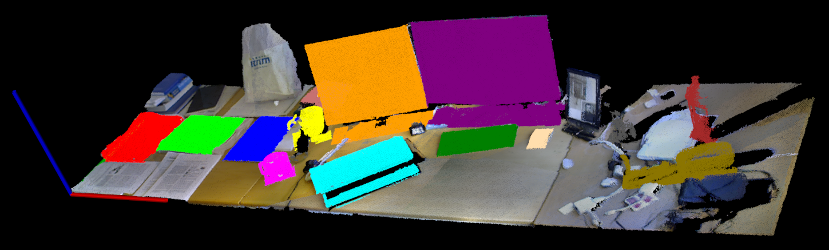
\includegraphics[scale=0.1]{pcd_annotated.png}}
\caption{(a) Objects annotated in 3D long-term dataset, sorted in descending order of count of occurrences. X-axis$=$Object Name, Y-axis$=$Occurrence Count. (b) Screenshot of one table scene, along with it's annotations in (c).}

\end{center}
\end{figure}

To enable us to develop and test our techniques for spatial-relation-based scene understanding, we have created a dataset of table-top scenes. To reflect our interest in long-term autonomy, this dataset contains views of the same tables captured periodically, across intervals of a few hours, over many days. The dataset therefore captures the individual and group variation in object position and pose due to human interaction. The required regularity in instances and time was the main motivation for the construction of this dataset, as currently available datasets either are of individual objects or singular instances of entire rooms\nick{can we cite these other datasets?}. 

% We need to be anonymous
% A 3D dataset " \textit{Tables for Spatial Modelling}" has been created by KTH, Royal Institute of Technology. 

The dataset is a collection of human-annotated office table scenes from a computer science research institute. The data was collected using the \textit{SCENECT} software \cite{Buerkler:Online2012} and an \textit{Asus Xtion Pro} RGB-D camera. Within the data, a \textit{Scene} is defined to be a single instance of a table-top of one person at a single instance in time. There is one 3D colour point cloud per scene (.pcd format). Every scene is a reconstructed version of the raw data stream obtained by a person scanning a table-top with real time visual feedback using SCENECT. The software has in-built real-time sampling, registration and de-noising algorithms to output the final high resolution point cloud.

The scenes were recorded as periodically as possible and at three fixed time instances of the day: \emph{Morning} (09:00 hrs), \emph{Afternoon} (13:00 hrs) and \emph{Evening} (18:00 hrs). Scenes for 20 different tables were collected for 19 days, 3 times per day. A \textit{Scene\_ID} is attached to each scene to indicate who the table belongs to and the date and time of the recording. These Scene\_IDs help in slicing across the dataset with respect to time of the day \{Morning, Afternoon, Evening\}, person \{Anna, Bob, Carl, \dots\}, or day \{2013-11-01, 2013-11-06, 2013-11-13, \dots\}.

A 3D annotation tool was developed for manually segmenting out objects of interest from the point clouds. On average, 12 different objects were labelled per scene. The objects belong to the following super set - \{Mouse, Keyboard, Monitor, Laptop, Cellphone, Keys, Headphones, Telephone, Pencil, Eraser, Notebook, Papers,  Book, Pen, Highlighter, Marker, Folder, Pen-Stand, Lamp, Mug, Flask, Glass, Jug, Bottle\}. The information about every scene and object is available in  XML and JSON formats. Each scene has a nested list of object data containing \{Position, Orientation, Size, Date and Time of recording, Person ID, Point Indices of the point cloud that have been labelled as belonging to the Object\}.

\ifdraft
\points{
\subsubsection*{Points Discussed}
\begin{enumerate}
	\item Details
	\item Why?
	\item Histogram of all objects in data set
	\item Scatter plot like in Adria thesis - centroids of objects and motivate learning that model.
\end{enumerate}
}
\fi

\section{Evaluation Scenario} % (fold)
\label{sec:evaluation_scenario}

\nick{add images of robot/scenes here} 

Our evaluation scenario stems from our interest in long-term autonomy in real environments. Our techniques will run on a mobile robot capable of patrolling a collection of offices a couple of times during the day\footnote{Whilst we have the majority of this system implemented and running, we exclude details here for blind review and space constraints}. The role of this robot is to inspect the tables in these offices for certain conditions (e.g. checking that laptops or confidential papers have not been left unattended in an insecure area). This robot is equipped with a 3D \textit{perception system} (PS) which can segment potential objects from table-top backgrounds as \emph{object clusters}. It can also use a pre-trained classifiers to assign a distribution over category labels to each cluster~\cite{aldoma2012using}. The task we now address is -- how can the spatial properties of the observed object clusters be used to improve the performance of the robot on this categorisation task beyond the baseline provided by the unaugmented classifier? We assume that the robot has access to a database of labelled table-top scenes, as would be captured on its previous patrols of the same offices, and must create a model from this data which it can exploit for the labelling. 

To provide a detailed exploration of approaches for representing and reasoning with spatial context, we remove the robot from the design and evaluation of techniques, and instead use the new dataset described above in place of the observations that would have, in principle, been gathered by the robot on previous patrols. Evaluating on a dataset rather than a real robot  allows us to vary parameters in the experimental configuration (e.g. initial classifier labelling accuracy) in order to consider a broader range of conditions that would otherwise be possible. However, our evaluation setup (Section~\ref{Experimental Setup}) is constrained to conditions that reflect the operation of the full robot system (e.g. the order in which the observations are gathered). 


% section evaluation_scenario (end)

\section{Metric and Qualitative Spatial Context}
\label{sec:Techniques}

The following sections present two approaches for learning spatial relation models (SRM) from observations of object configurations. The first approach (Section~\ref{sec:metric}) is based on metric information, the second (Section~\ref{sec:qsr}) abstracts from metric information to qualitative relations. Whilst the metric approach is based on state-of-the-art features it produces a model which is useful only for object class inference. The qualitative approach creates a representation which can be reused for a broader a range of spatial tasks (including grounding language), but its coarser representational structure may prevent it from making certain distinctions during inference. 

\subsection{Metric Spatial Relations}\label{sec:metric}

Joint object classification is performed using a voting scheme based strategy that captures the spatial and semantic coherence of object arrangements in an indoor scene environment by exploring the spatial relations of objects.

\paragraph{Spatial Features and Spatial Relation Based Features}

To model the object categories and the relationships between pairs of object categories, we use the sets proposed in \cite{alberti:2014} to capture the object geometry and the spatial distribution of objects in the scene. \emph{Single object features} (SOF) $f_{o_{i}}$, where $o_{i}$ is the $i^{th}$ object, are computed from the 3D spatial characteristics of the object w.r.t. a reference frame and origin (here the table and its front-left corner). The set features consists of: the projected lengths of the object along the X, Y and Z reference axes; 3D coordinates of the object centroid; horizontal bearing of the object centroid from front-left table corner. \emph{Object pair features} (OPF) represent the pairwise spatial distribution of the objects, $f_{o_{i},o_{j}}$ as: Euclidean distance between object centroids and it's projection in the X-Y plane; bearing between the two object centroids; ratio of object volumes; vertical displacement between object centroids.

\paragraph{Learning Spatial Models}

In the training phase, a set of models for each of the object class categories are learned by using a Gaussian Mixture Model (GMM)-based representation to encode the multivariate probability distribution of \emph{SOF}. The relationship of the different object category pairs are modelled by applying a GMM on the multi-dimensional feature space of \emph{OPF} set.

\paragraph{The Voting Scheme}

In the inference phase, a voting scheme is applied and a score $Score_{A}(o_{i}, c_{p})$, is computed for the assignment of each test object, $o_{i}$, to each of the possible categories, $c_{p}$, based on the spatial relations with the reference system and with the other objects and on typical object occurrence and co-occurrences. $Score_{A}(o_{i}, c_{p})$ is computed as the sum of \emph{pairwise scores} that involve the considered assignment:

\begin{multline}
Score_{A}(o_{i}, c_{p}) = \\ 
				\sum_{\substack{j \in \{1,\dots,n\} \\ j \neq i} } \sum_{\substack{q \in \{1,\dots,m\} \\ q \neq p}} 
                                 Score_{P}((o_{i}, c_{p}), (o_{j}, c_{q})), 
\label{eq:totalScore}
\end{multline}

\noindent where $n$ is the number of test objects and $m$ is the number of object categories. The \emph{pairwise score} is defined as:

\begin{multline}
Score_{P}((o_{i}, c_{p}), (o_{j}, c_{q})) = Score_{SO}(o_{i}, c_{p}) \cdot \\ Score_{SO}(o_{j}, c_{q}) \cdot Score_{OP}((o_{i}, o_{j}), (c_{p}, c_{q})).
\end{multline}

The scores $Score_{SO}(o_{i}, c_{p})$ and $Score_{OP}((o_{i}, o_{j}), (c_{p}, c_{q}))$ take into account the likelihood values of the category models and the likelihood value of the category pair model -- given the extracted features, corresponding to the conditional probability of the features -- given the trained models. Additionally, the scores integrate, as a-priori weights, the occurrence probability of the individual object categories and the co-occurrence probability of the object category pairs, estimated using frequency counts on the training database. The confidence or probability value provided by a vision based PS, $C_{perc}(o_{i}, c_{p})$, is also considered when it is available, as follows:

\begin{equation}
Score_{SO}(o_{i}, c_{p}) = Pr(f_{o_{i}}|c_{p})  \cdot \frac{max(1, N_{c_{p}})}{(1 + N_{tot})} \cdot C_{perc}(o_{i}, c_{p}),
\label{eq:scoreSO}
\end{equation}

\begin{multline}
Score_{OP}((o_{i}, o_{j}), (c_{p}, c_{q})) = Pr(f_{o_{i},o_{j}}|c_{p}, c_{q})  \cdot \\ \frac{max(1, N_{c_{p}, c_{q}})}{(1 + N_{tot})},
\end{multline}

\noindent where $N_{c_{p}}$ is the number of training scenes where $c_{p}$ is present, $N_{c_{p}, c_{q}}$ is the number of scenes where both $c_{p}$ and $c_{q}$ are present and $N_{tot}$ is the total number of training scenes. The numerator and denominator terms, $max(1, N_{c_{p}})$, $max(1, N_{c_{p}, c_{q}})$ and $(1 + N_{tot})$, ensure that occurrence and co-occurrence weights are never $0$ or $1$.

%%%%%%%%%%%%%%%%%%%%%%%%%%%%%%%%%%%%%%%%%%%%%%%%%%%%%%%%%%%%%%%%%%%%%%%%%%%%%%%%%%%%%%%%

\subsection{QSR-based technique}\label{sec:qsr}

Qualitative relational approaches abstract away the geometric information of a scene such as relative angles, relative distances, and relative sizes, and instead represent a scene using first-order predicates such as \emph{left-of}, \emph{close-to}, and \emph{smaller-than}. Our work first generates these first-order predicates from geometric descriptions, then builds a probabilistic model to reason about the class of an object, without knowing the geometric grounding of the state.

\subsubsection{Qualitative Relations}

In this work we adopt a semi-supervised approach to generating spatial relation predicates which combines a geometric calculus with clustering methods. This produces a symbolic description of a geometric configuration constructed from $12$ predicates: $4$ directional, $3$ distance, $3$ size and $2$ projective.

\textbf{Directional} predicates are created using the \emph{ternary point calculus}~\cite{Moratz:2003ti}. The three positions in the calculus are the \emph{origin}, \emph{relatum} and \emph{referent}. In this work, \emph{origin} corresponds to the position of the robot, \emph{relatum} to a landmark object, and the \emph{referent} to another object under consideration. In the following we denote these positions by \emph{robot}, \emph{landmark}, and \emph{object}. \emph{Robot} and \emph{landmark} define the reference axis which partitions the surrounding space. Then, the spatial relation is defined by the partition in which \emph{object} lies with respect to the reference axis. In order to determine the partition, i.e. the directional relation, we calculate the relative angle $\phi_{rel}$ as follows:

\begin{equation}
  \phi_{rel} = \tan^{-1} \frac{y_{obj} - y_{land}}{x_{robj} - x_{land}} - \tan^{-1} \frac{y_{land} - y_{robot}}{x_{land} - x_{robot}}
\end{equation}

\noindent $\phi_{rel}$, is the angle between the reference axis, defined by \emph{robot} and \emph{landmark}, and the \emph{object} point. Dependent on this angle we assign directional relations (\emph{behind, in-front-of, left-of, right-of}) to pairs of objects.

\textbf{Distance} relations are determined by clustering observed geometric examples. A training set of object scenes is used to derive cluster boundaries between a previously defined number of clusters, each of which will correspond to a  qualitative relation. Based on the membership of a geometric relation to a cluster, the associated qualitative predicate is then assigned to a pair of objects. In our technique we use three different predicates: \emph{very-close-to, close-to, distant-to}.

\textbf{Size} predicates compare the bounding box dimensions of two objects. Each axis is compared individually, leading to the three predicates \emph{shorter-than}, \emph{narrower-than}, and \emph{thinner-than}.

\textbf{Projective connectivity} between two objects uses uses Allen's interval calculus~\cite{Allen83} on the projection of the objects' axis-aligned bounding boxes onto the x or y axis. The `\emph{overlaps} predicate is then extracted for each axis. 



\subsubsection{Probabilistic QSR-based Reasoning}

Our objective is to infer the types of all objects given a symbolic scene description 
\begin{equation}
  S=C_1 \wedge C_2 \wedge ... \wedge C_n
\end{equation}
where $C_n$ is a clause in a description comprising of a relation predicate $R$ between two objects $O_A$ and $O_B$:
\begin{equation}
C_n = (R\,\,\,\, O_A\,\,\, O_B),
\end{equation}
for example \texttt{(shorter-than object15 object7)}.

To achieve this we formulate the problem probabilistically: from a training set of scene descriptions for which object types are labelled, we use the occurrence count for each relation to estimate the probability that it will hold given the object types of its arguments:
\begin{equation}
p(R_n^{AB} | L_A, L_B)=\frac{N_{R_n,L_A,L_B}}{N_{L_A,L_B}}
\end{equation}
where $R_n^{AB}$ is one of the $12$ symbolic relations between two objects $O_A$ and $O_B$ with class labels  $L_A, L_B$, $N_{L_A,L_B}$ is the number of times that objects of types $L_A$ and $L_B$ have co-occurred across all training scenes, and $N_{R_n,L_A,L_B}$ is the number of times that relation $R_n$ has occurred between objects of types $L_A$ and $L_B$ across all training scenes.

Then, given a new scene description $S$ for which the object types are only known from perception with a certain confidence, we find all object labels simultaneously. Assuming that one relation holding is independent of another holding, we can apply Bayes theorem recursively to find the labels of all objects:

\begin{equation}\label{eq:l-given-rels}
p(L | R_1, R_2 ... R_n) \propto \prod_{i=1..n} p(R_i | L) p(L)
\end{equation}
where $L$ is a vector of class labels for the objects in $S$, and $R_i$ is the $i$th relation in $S$. The prior probability of the labels $p(L)$ comes from the robot's perception model: 

\begin{equation}
p(L)=\prod_{i=1..n}p(L_n)
\end{equation}
where all $n$ object class labels are independent and provided with their confidences $p(L_n)$.

Finding the optimum class labelling estimate $\hat{L}$ for the objects is then equivalent to finding the maximum posterior in Equation~\ref{eq:l-given-rels}. To avoid computational arithmetic problems when dealing with very small unnormalised probabilities, we replace the product in Equation~\ref{eq:l-given-rels} with a sum of logarithms:
\begin{equation}
\hat{L}=\operatorname*{arg\,max}_L \sum_{i=1..n} \log p(R_i | L)  \log p(L)
\end{equation}

\noindent We performed this maximisation using gradient ascent.

\section{Experimental Evaluation}
\label{Experimental Evaluation}

\subsection{Experimental Setup}
\label{Experimental Setup}

To compare the above approaches on the task of improving object labelling using spatial context we use the following experimental setup. The annotated dataset is split into training and test sets as described below. For the test data we use a simulated PS to assign class labels to objects along with confidence values. We can configure this simulated PS with a perceptual accuracy percentage ($PA$), which describes the percentage of objects which are assigned the correct label. We varied this percentage to explore how different perceptual systems will benefit from our work. We also varied the percentage of the available training data ($TP$) we used to train our models, to explore how sensitive the approaches are to data availability -- as this is crucial in online learning applications (such as our long-term autonomous patrolling robot).

Using this setup we performed two experiments with different foldings of the data: \textit{leave one out foldings} (LOOF) and \textit{single table foldings} (STF). The LOOF experiments evaluate how our approaches operate on unseen tables (the ones left out) after training on all other tables. This is to replicate the condition of a trained robot encountering a new table, a likely situation in our application. The STF experiments evaluate how our approaches perform on a single person's table over time. This is also an important use case on our robot, where data from individual tables can be separated by position in a global map. For the LOOF experiments we split the data 70/30 into train and test sets (14/6 tables or 688/295 scenes), performing 4 folds, each fold the 6 left out tables randomly selected. For STF we split the data 60/40, working with 36/24 scenes per table, with results averaged over 6 tables. In all cases we tested $PA$ values of 0\%, 25\%, 50\%, 75\% and 100\%, and $TP$ values of 10\%, 60\% and 100\% (of the assigned training set). For each experiment we apply both the metric spatial model from Section~\ref{sec:metric} (labelled SM below) and the qualitative model from Section~\ref{sec:qsr}. For this latter technique we explore the effects of different combinations of qualitative relations. Individual relations are labelled as follows: ternary point calculus (T), qualitative distance (D), relative size (R), projective connectivity (C). Combinations of labels reflect the combination of relations that were employed (e.g. TDRC uses all relations).

\subsection{Results and Analysis}
\label{sec:Analysis}

\begin{figure}[t]
\begin{center}
\subfloat[][]{\label{fig:resultsLOOF:a}\includegraphics[scale=0.4]{LOOF1_Second_raw_crp.pdf}}\\
\subfloat[][]{\label{fig:resultsLOOF:b}\includegraphics[scale=0.21]{LOOF2_First_raw_crp.pdf}}\quad
\subfloat[][]{\label{fig:resultsLOOF:c}\includegraphics[scale=0.21]{LOOF2_Second_raw_crp.pdf}}
\caption{Comparison of our spatial relation models (SRM) with different testing parameters. X-axis$=$PA, Y-axis$=$PS+SRM accuracy. (a) SM(\textcolor{OliveGreen}{\textbf{$\bullet$}}), TDRC(\textcolor{Red}{\textbf{$\bullet$}}), TDR(\textcolor{blue}{\textbf{$\bullet$}}), TD(\textcolor{Violet}{\textbf{$\bullet$}}) and T(\textcolor{Sepia}{\textbf{$\bullet$}}) techniquess trained at 60\% of training fold.(b) SM technique at different TPs. (c) TDRC technique at different TPs. TP $=$ 10\%(\textcolor{OliveGreen}{\textbf{$\bullet$}}) 60\%(\textcolor{red}{\textbf{$\bullet$}}) 100\%(\textcolor{blue}{\textbf{$\bullet$}}) in (b,c). The error bars in all, capture the $\max$ and $\min$ value of the PS+SRM system accuracy when checked for different foldings. Raw PS system accuracy is in ({$\bullet$}).}

\label{fig:resultsLOOF}

\end{center}
\end{figure}

Figure~\ref{fig:resultsLOOF:a} presents the comparison of all our techniques with respect to changes in the accuracy of the perceptual system (PA). The results show that for low perceptual accuracy, all approaches offer an improvement beyond perception, but as perceptual accuracy increases the effect lessens, with only the SM approach offering any improvement when the perceptual accuracy reaches 75\%. Our different techniques encode different amounts of information about scene context. SM has the most information (including spatial relations plus size-object size and location features) and commensurately makes the most improvement over raw perception. As additional relations (and thus information) are added to the qualitative relational approaches, a corresponding performance increase occurs, although it appears that the connectivity relation does not have any effect on the data. With perceptual accuracy at 0\% it is clear that spatial information alone is sufficient to achieve reasonable classification accuracy for some techniques (SM, TDR(C)), and at 100\% all of the techniques correctly trust perception and do not reduce the combined accuracy. This is not the case for the T(D) approaches at 50\% and 75\% perceptual accuracy, where they actually reduce the combined result below raw perception.  Figures~\ref{fig:resultsLOOF:b} and ~\ref{fig:resultsLOOF:c} demonstrate the influence of the amount of training data on our techniques (TP). There is very small incremental change in performance as the training set ranges from 10\% to 100\% of the available training data.

\begin{figure}[t]
\begin{center}
\subfloat[][]{\label{fig:resultsSTF:a}\includegraphics[scale=0.235]{STF_TP10_raw_crp.pdf}}\quad
\subfloat[][]{\label{fig:resultsSTF:b}\includegraphics[scale=0.235]{STF_TP60_raw_crp.pdf}}
\caption{Comparison of our spatial relation models (SRM) with different testing parameters. X-axis$=$PA, Y-axis$=$PS+SRM accuracy. (a) SM(\textcolor{OliveGreen}{\textbf{$\bullet$}}), TDRC(\textcolor{Red}{\textbf{$\bullet$}}), TDR(\textcolor{blue}{\textbf{$\bullet$}}), TD(\textcolor{Magenta}{\textbf{$\bullet$}}) and T(\textcolor{Sepia}{\textbf{$\bullet$}}) techniquess trained at 60\% of training data and (b) 10\% of training data. The error bars capture the $\max$ and $\min$ value of the PS+SRM system accuracy when checked for different tables. Raw PS system accuracy is in ({$\bullet$}).}

\label{fig:resultsSTF}
\end{center}
\end{figure}

Figure~\ref{fig:resultsSTF:a}, shows the results of the STF experiments. As these were performed  on only data from a single table, much less data was available in each case (100\% $TP$ is 36 scenes). When only very few training samples are available (Figure~\ref{fig:resultsSTF:b}) the SM model is unable to generalise, whereas the QSR models perform adequately, benefiting from the natural generalisation of their coarser representation. In cases where mode data is available, the results show a similar pattern to the LOOF experiments, with the more detailed model of SM outperforming the QSR approaches. Overall, these are good results for the real robot where it must start from little or no knowledge and learn online from its observations. It seems reasonable that the robot could start from a QSR-based model while gathering initial data, before switching to an SM model when its performance starts to overtake that of QSRs.

\section{Conclusions}
\label{sec:Conclusions}

We presented two techniques for learning spatial context from observations of collections of objects, and for using this learnt context to improve the performance of a perceptual system on an object classification task. Our techniques were evaluated on a novel long-term 3D table-top dataset. The results showed that spatial context knowledge can be used to improve classification results beyond that of raw perception, and that different models can play different roles in a robot system: more complex metric models using both single-object and relational features appear to ultimately have better performance when enough training data is available to allow them to generalise, but coarser qualitative relational still perform when only few training samples are available. In the future we plan to extend this research to beyond table-top scenes to full rooms, and evaluate similar techniques in an online, active learning setting to the real robot.


\ifdraft
\points{
\subsubsection*{Points Discussed}
\begin{enumerate}
	\item Room level data set
	\item Which QSR for which purpose?
\end{enumerate}
}
\fi
% \section{Acknowledgements}
% \label{sec:Acknowledgements}
% We would like to heartily thank the following people and organizations without whom the above work could not have been completed. Adria Gallart Del Burgo, Kaushik Desai, Malepati Bala Siva Sai Akhil, Gaurav Agrawal, Janardhan HR, Mayank Jha, Nishan B Shetty, Prasad NR, Shekhar Kirani - Accel Partners, Dept of Telecommunication - MSRIT Bangalore, STRANDS project, SSF through its Centre for Autonomous Systems.
\clearpage
\bibliographystyle{aaai}
\bibliography{references}

\end{document}
